\begin{frame}
    \frametitle{Visualizzare ed Elaborare documenti XML}
    \addtocounter{nframe}{1}
    
    %\begin{center}
    %    
\includegraphics[width=.2\textwidth]{../imgs/tei-r.pdf}
    %\end{center}
    %\textit{In parte già disponibili nei moduli TEI di base}

     \begin{block}{Documenti Object Model (DOM)}
        Il \textbf{Document Object Model} (\textit{DOM}) è un modello \textit{language-independent} che mette a disposizione delle \textbf{Application Programming Interface} (\textit{API}) per accedere e manipolare documenti XML (e HTML).

     \end{block}

     \begin{block}{Documenti Object Model (DOM)}
        Il Modello DOM rappresenta l'intero documento XML come una gerarchia di nodi (\textit{albero}).
     \end{block}


\end{frame}


\begin{frame}
    \frametitle{Visualizzare ed Elaborare documenti XML}
    \addtocounter{nframe}{1}
    \textit{Esempio albero DOM}    
    \begin{center}
        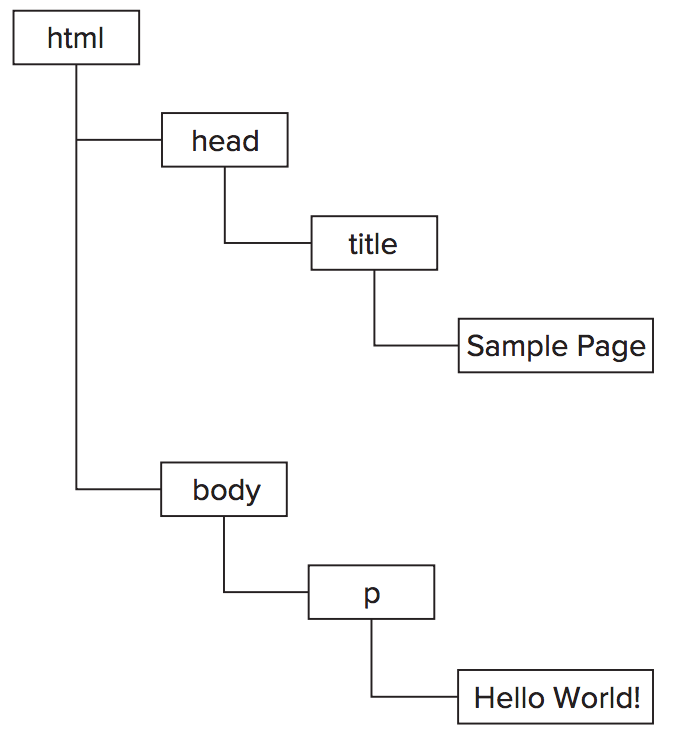
\includegraphics[width=.6\textwidth]{imgs/XML-DOM.png}
    \end{center}

\end{frame}

\begin{frame}
    \frametitle{Visualizzare ed Elaborare documenti XML}
    \addtocounter{nframe}{1}
    
    %\begin{center}
    %    
\includegraphics[width=.2\textwidth]{../imgs/tei-r.pdf}
    %\end{center}
    %\textit{In parte già disponibili nei moduli TEI di base}

     \begin{block}{Documenti Object Model (DOM)}
        Ciascuna parte di un documento XML-TEI è quindi un tipo specifico di nodo DOM costituito da diversi tipi di dati.
     \end{block}

     \begin{block}{Documenti Object Model (DOM)}
        Grazie alla rappresentazione gerarchica messa a disposizione dal DOM è possibile avere un livello di controllo a granularità molto fine per manipolare quasi tutti gli aspetti del documento XML originario.
     \end{block}
     
\end{frame}

\begin{frame}
    \frametitle{Visualizzare ed Elaborare documenti XML}
    \addtocounter{nframe}{1}
    
    %\begin{center}
    %    
\includegraphics[width=.2\textwidth]{../imgs/tei-r.pdf}
    %\end{center}
    %\textit{In parte già disponibili nei moduli TEI di base}

     \begin{block}{Documenti Object Model (DOM): espressività}
       I nodi di un albero DOM possono essere aggiunti, modificati, cancellatti o rimpiazzati facilmente frazie alle API definite dal modello.
     \end{block}

     \begin{block}{Documenti Object Model (DOM)}
        Il modello DOM è una specifica e una raccomandazione del consorzio di standardiziazione Web W3C.
        \\\url{URL/TO/DOM/W3C/RECOMMENDATION}
     \end{block}
     
\end{frame}

\begin{frame}
    \frametitle{Visualizzare ed Elaborare documenti XML}
    \addtocounter{nframe}{1}
    
    %\begin{center}
    %    
\includegraphics[width=.2\textwidth]{../imgs/tei-r.pdf}
    %\end{center}
    %\textit{In parte già disponibili nei moduli TEI di base}

     \begin{block}{Documenti Object Model (DOM): Browser-Indipendent}
        Una importante caratteristica del Modello e delle API DOM è la sua indipendenza dalla tecnologia di implementazione.
        
     \end{block}

     \begin{block}{Tecnologia indipendente dal software}
        Un importante obiettivo dello standard DOM è quello di essere cross-platform. 
        \\In realtà però non tutti i browser implementano con le stesse modalità le specifiche, così come non tutti i browser sono allineati all'ultima versione del modello (copertura non al 100\%).
       
     \end{block}
     
\end{frame}


\begin{frame}
    \frametitle{Visualizzare ed Elaborare documenti XML}
    \addtocounter{nframe}{1}
    
    %\begin{center}
    %    
\includegraphics[width=.2\textwidth]{../imgs/tei-r.pdf}
    %\end{center}
    %\textit{In parte già disponibili nei moduli TEI di base}

     \begin{block}{DOM Levels}
       Esistono diverse versioni (livelli) dello standard DOM nonché diverse moduli all'interno di ciascun livello.
     \end{block}

     \begin{block}{DOM Levels}
       Allo stato attuale, il Modello DOM conta 5 diverse versioni o approcci (livelli), a loro volta suddivisi in sezioni o aree.
     \end{block}
     
\end{frame}

\begin{frame}
    \frametitle{Visualizzare ed Elaborare documenti XML}
    \addtocounter{nframe}{1}
    
    %\begin{center}
    %    
\includegraphics[width=.2\textwidth]{../imgs/tei-r.pdf}
    %\end{center}
    %\textit{In parte già disponibili nei moduli TEI di base}

     \begin{block}{le API con il linguaggio di programmazione javascript}
       E' possibile sfruttare, anche attraverso javascript nativo, la rappresentazione ad albero di un documento XML e le funzionalità che DOM mette a disposizione per accedere, manipolare ed estrarre informazioni da un documento XML.
     \end{block}
     
\end{frame}


\begin{frame}
    \frametitle{Visualizzare ed Elaborare documenti XML}
    \addtocounter{nframe}{1}
    
    %\begin{center}
    %    
\includegraphics[width=.2\textwidth]{../imgs/tei-r.pdf}
    %\end{center}
    %\textit{In parte già disponibili nei moduli TEI di base}

     \begin{block}{DOM Level 0}
       \textbf{Il livello 0} del DOM indica la madalità 'legacy' di operare sui documenti, sarebbe cioè quella che non tiene di conto delle specifiche W3C.
     \end{block}
     

     \begin{block}{DOM Level 0}
        Adottando DOM Level 0 si suppongono anche scelte imiplementative non cross-platform e non browser-independent.
      \end{block}

\end{frame}

\begin{frame}
    \frametitle{Visualizzare ed Elaborare documenti XML}
    \addtocounter{nframe}{1}
    
    %\begin{center}
    %    
\includegraphics[width=.2\textwidth]{../imgs/tei-r.pdf}
    %\end{center}
    %\textit{In parte già disponibili nei moduli TEI di base}

     \begin{block}{DOM Level 1}
       \textbf{DOM Level 1} è la prima versione dello standard (\textit{raccomandazione W3C nel 1998}). 
       \\ La specifica definisce  \textbf{oggetti, proprietà e funzionalità di base} per navigare e manipolare la struttura di un documento XML (e HTML).
     \end{block}

\end{frame}


\begin{frame}
    \frametitle{Visualizzare ed Elaborare documenti XML}
    \addtocounter{nframe}{1}
         
     \begin{block}{DOM Level 1}
        Il DOM Level 1 è diviso in due sezioni:
        \begin{itemize}
            \item[1] \textbf{Generica} per la gestione di documenti XML e HTML
            \item[2] \textbf{Specifica} per documenti HTML: questa sezione estende la prima (Sezione Generale).
        \end{itemize}
      \end{block}

\end{frame}

\begin{frame}
    \frametitle{Visualizzare ed Elaborare documenti XML}
    \addtocounter{nframe}{1}
    
    %\begin{center}
    %    
\includegraphics[width=.2\textwidth]{../imgs/tei-r.pdf}
    %\end{center}
    %\textit{In parte già disponibili nei moduli TEI di base}

     \begin{block}{DOM Level 2}
       \textbf{DOM Level 2} è una estensione del livello 1 e aggiunge a quest'ultimo numerose funzionalità e moduli specifici, come per esempio la gestione degli eventi e dei fogli di stile CSS.
     \end{block}
     

     \begin{block}{DOM Level 2}
       Tra i vari moduli che \textit{DOM Level 2} aggiunge, di particolare interesse è il modulo \textbf{DOM Traversal and Range}.
      \end{block}

\end{frame}

\begin{frame}
    \frametitle{Visualizzare ed Elaborare documenti XML}
    \addtocounter{nframe}{1}
    
    %\begin{center}
    %    
\includegraphics[width=.2\textwidth]{../imgs/tei-r.pdf}
    %\end{center}
    %\textit{In parte già disponibili nei moduli TEI di base}

     
      \textbf{Lo standard \textit{DOM Level 3} ha raggiunto lo status di raccomandazione W3C nel 2004.}
     

     \begin{block}{DOM Level 3}
        \begin{itemize}
            \item Migliora ed estende il modulo di gestione degli eventi definito nel DOM Level 2
            \item Aggiunge funzionalità per \textit{supportare tutta la specifica della versione 1.0} di XML (es.: \textbf{XML namespace}, \textbf{XPath}, \textbf{DOM Validaton})
            \item Caricamento e salvataggio dei documenti con serializzazione XML (\textbf{DOM Load and Save}).
        \end{itemize}
       
      \end{block}

\end{frame}


\begin{frame}
    \frametitle{Visualizzare ed Elaborare documenti XML}
    \addtocounter{nframe}{1}
    
    %\begin{center}
    %    
\includegraphics[width=.2\textwidth]{../imgs/tei-r.pdf}
    %\end{center}
    %\textit{In parte già disponibili nei moduli TEI di base}

     \begin{block}{DOM Level 4}
     \textbf{DOM Level 4} è la prossima versione del Modello DOM sulla quale sta lavorando il W3C. Ancora non ha raggiunto lo status di raccomandazione e non è ancora supportata dai browser. 
     \end{block}
     
\end{frame}

\begin{frame}
    \frametitle{Visualizzare ed Elaborare documenti XML}
    \addtocounter{nframe}{1}
    
    %\begin{center}
    %    
\includegraphics[width=.2\textwidth]{../imgs/tei-r.pdf}
    %\end{center}
    %\textit{In parte già disponibili nei moduli TEI di base}

     \begin{block}{Supporto dei browser alle specifiche DOM}
        Da qualche anno il supporto alle specifiche e alle API DOM è \textbf{diventato una priorità}, oltre che una necessità, per i più grossi gruppi che sviluppano browser.
        \\ Tuttavia non tutte le principali compagnie implementano allo stesso modo lo standard.
     \end{block}
     
\end{frame}


\begin{frame}
    \frametitle{Visualizzare ed Elaborare documenti XML}
    \addtocounter{nframe}{1}
    
     \begin{block}{Il Modello DOM in sistesi}
        \begin{itemize}
            \item Un documento XML può essere rappresentato come una gerarchia di nodi attraverso il modello DOM.
            \item Ciascun tipo di nodo ha caratteristiche, dati e funzionalità differenti.
            \item Caiascun tipo di nodo può avere differenti tipi di relazioni con gli altri tipi di nodi.
            \item Le relazioni tra i nodi DOM creano una gerarchia, la quale permette di rappresentare un documento XML come un albero.
        \end{itemize}
     \end{block}
     
\end{frame}

\begin{frame}
    \frametitle{Visualizzare ed Elaborare documenti XML}
    \addtocounter{nframe}{1}
    
    %\begin{center}
    %    
\includegraphics[width=.2\textwidth]{../imgs/tei-r.pdf}
    %\end{center}
    %\textit{In parte già disponibili nei moduli TEI di base}

     \begin{block}{Il Modello DOM: principali caratteristiche}
        \begin{itemize}
            \item Il Modello DOM ha un nodo \textbf{document} che rappresenta tutto il documento attraverso la cosiddetta \textbf{radice} del documento.
            \item Il Modello DOM ha un elemento detto document element che è l'elemento più esterno del documento, il quale è avo di tutti gli altri elementi e che quindi li racchiude tutti. (esiste solo un \textit{document element} per documento)
            \item Ciascun pezzo del documento XML può essere rappresentato da un nodo DOM in un albero DOM.
        \end{itemize}
     \end{block}
     
\end{frame}

\begin{frame}
    \frametitle{Visualizzare ed Elaborare documenti XML}
    \addtocounter{nframe}{1}
    
    %\begin{center}
    %    
\includegraphics[width=.2\textwidth]{../imgs/tei-r.pdf}
    %\end{center}
    %\textit{In parte già disponibili nei moduli TEI di base}

     \begin{block}{Il Modello DOM: principali caratteristiche}
        \begin{itemize}
            \item A differenza di XSLT, DOM presenta 12 node types, ciascuno dei quali eredita da un nodo di base (in js tutto il data model parte dall'interfaccia \textit{Node Type}).
            \item Ciascun nodo ha una proprietà che indica il tipo del nodo stesso (in js nodeType)
        \end{itemize}
     \end{block}
     
\end{frame}

\begin{frame}
    \frametitle{Visualizzare ed Elaborare documenti XML}
    \addtocounter{nframe}{1}
    
    %\begin{center}
    %    
\includegraphics[width=.2\textwidth]{../imgs/tei-r.pdf}
    %\end{center}
    %\textit{In parte già disponibili nei moduli TEI di base}

     \textit{I tipi di nodo nel modello DOM}

        \begin{center}
            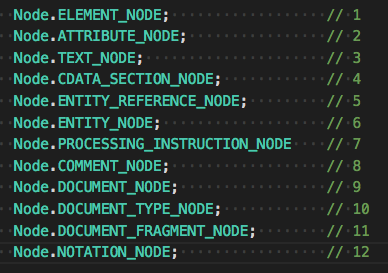
\includegraphics[width=.85\textwidth]{imgs/nodetypes.png}
        \end{center}
     
\end{frame}

\begin{frame}
    \frametitle{Visualizzare ed Elaborare documenti XML}
    \addtocounter{nframe}{1}
    
    %\begin{center}
    %    
\includegraphics[width=.2\textwidth]{../imgs/tei-r.pdf}
    %\end{center}
    %\textit{In parte già disponibili nei moduli TEI di base}

     \begin{block}{Il Modello DOM: principali caratteristiche}
        \begin{itemize}
            \item Tutti i nodi in un documento DOM instaurano relazioni gerarchiche tra di loro.
            \item Ciascun nodo ha una proprietà \textit{childNodes} contenente una lista di nodi, detta \textit{NodeList}.
        \end{itemize}
     \end{block}

     \begin{block}{Il Modello DOM: principali caratteristiche}

            Un oggetto NodeList è simile ad un array usato per memorizzare una lista ordinata di nodi accessibili per posizione
       
     \end{block}

\end{frame}

\begin{frame}
    \frametitle{Visualizzare ed Elaborare documenti XML}
    \addtocounter{nframe}{1}
    
    %\begin{center}
    %    
\includegraphics[width=.2\textwidth]{../imgs/tei-r.pdf}
    %\end{center}
    %\textit{In parte già disponibili nei moduli TEI di base}

     \begin{block}{Il Modello DOM: esempio NodeList}
        \texttt{firstChild = someNode.childNodes[0];}
        \\\texttt{secondChild = someNode.childNodes.item(1); }
        \\\texttt{count = someNode.childNodes.length;}
     \end{block}

\end{frame}

\begin{frame}
    \frametitle{Visualizzare ed Elaborare documenti XML}
    \addtocounter{nframe}{1}

    \textbf{Le relazioni di un nodo}
    
    \begin{center}
        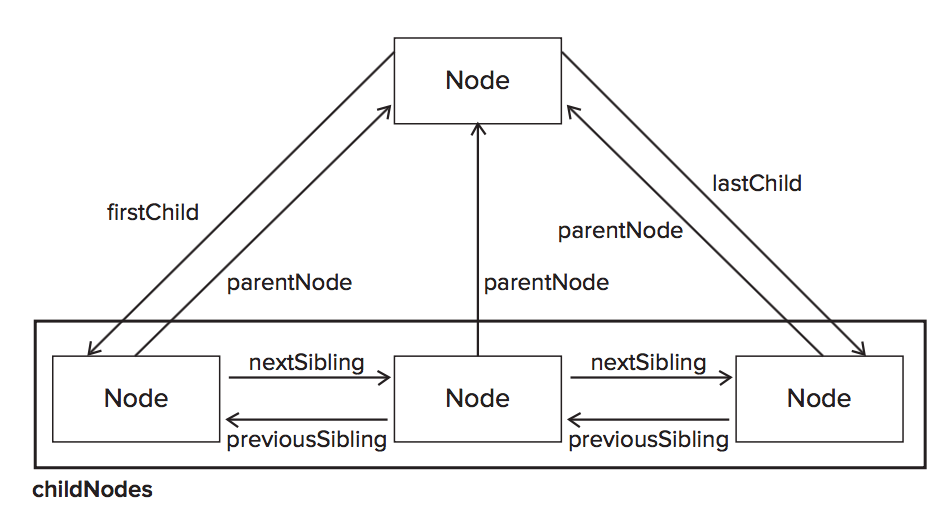
\includegraphics[width=.9\textwidth]{imgs/nodeRelations.png}
    \end{center}
    %\textit{In parte già disponibili nei moduli TEI di base}

\end{frame}

\begin{frame}
    \frametitle{Visualizzare ed Elaborare documenti XML}
    \addtocounter{nframe}{1}
    
    %\begin{center}
    %    
\includegraphics[width=.2\textwidth]{../imgs/tei-r.pdf}
    %\end{center}
    %\textit{In parte già disponibili nei moduli TEI di base}

     \begin{block}{Il Modello DOM: proprietà ownerDocument}
        Tutti i nodi condividono la proprietà \texttt{ownerDocument} che è un collegamento diretto al nodo che rappresenta l'intero documento.
     \end{block}

     \begin{block}{Il Modello DOM: proprietà ownerDocument}
        La proprietà \textit{ownerDocument} fornisce un modo veloce per accedere al \textit{nodo documento} senza dover attraversare tutta la gerachia di nodi per arrivare alla radice dell'albero.
     \end{block}

\end{frame}

\begin{frame}
    \frametitle{Visualizzare ed Elaborare documenti XML}
    \addtocounter{nframe}{1}
    
    %\begin{center}
    %    
\includegraphics[width=.2\textwidth]{../imgs/tei-r.pdf}
    %\end{center}
    %\textit{In parte già disponibili nei moduli TEI di base}

     \begin{block}{Il Modello DOM: metodi per la manipolazione}
        Una serie di metodi sono disponibili per la manipolazione dei nodi dell'albero DOM.
     \end{block}

     \begin{block}{Il Modello DOM: metodi per la manipolazione}
        Quattro di questi metodi (sei in totale) lavorano sui figli di uno specifico nodo.
        \\Poiché non tutti i tipi di nodi hanno nodi figli, questi ultimi metodi possono lanciare degli errori se invocati.
     \end{block}

\end{frame}

\begin{frame}
    \frametitle{Visualizzare ed Elaborare documenti XML}
    \addtocounter{nframe}{1}
    
    %\begin{center}
    %    
\includegraphics[width=.2\textwidth]{../imgs/tei-r.pdf}
    %\end{center}
    %\textit{In parte già disponibili nei moduli TEI di base}

     \textit{Il Modello DOM: metodi per la manipolazione}
       
    \begin{center}
        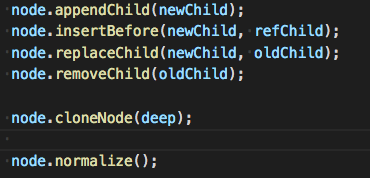
\includegraphics[width=.9\textwidth]{imgs/nodeManipulation.png}
    \end{center}
     
\end{frame}


%% piccolo approfondimento su Document Type - Element Type - Text Type - Attribute Type

\begin{frame}
    \frametitle{Visualizzare ed Elaborare documenti XML}
    \addtocounter{nframe}{1}
    
    %\begin{center}
    %    
\includegraphics[width=.2\textwidth]{../imgs/tei-r.pdf}
    %\end{center}
    %\textit{In parte già disponibili nei moduli TEI di base}

     \begin{block}{Il Modello DOM: Document Type}
        \begin{itemize}
            \item Rappresenta un intero documento ed è la radice della gerarchia.
            \item L'oggetto \textit{document} è una istanza di tipo \textbf{Document}, attraverso di esso è possibile interrogare e ottenere altri nodi in molti modi diversi.
        \end{itemize}
     \end{block}

     \begin{block}{Il Modello DOM: Document Type esempio}

            \texttt{xmlRootElement = document.documentElement;}
            \\\texttt{divElement = document.getElementById('divID');}
            \\\texttt{myDivList = document.getElementsByTagName('div');}
       
     \end{block}

\end{frame}

\begin{frame}
    \frametitle{Visualizzare ed Elaborare documenti XML}
    \addtocounter{nframe}{1}
    
    %\begin{center}
    %    
\includegraphics[width=.2\textwidth]{../imgs/tei-r.pdf}
    %\end{center}
    %\textit{In parte già disponibili nei moduli TEI di base}

     \begin{block}{Il Modello DOM: Element Type}
        \begin{itemize}
            \item Rappresenta elementi XML (ma anche HTML) in un documento
            \item Usato per accedere e manipolarne il contenuto e/o il valore dei propri attributi 
        \end{itemize}
     \end{block}

     \begin{block}{Il Modello DOM: Element Type esempio}

        \texttt{myDiv.tagName == myDiv.nodeName}
        \\\texttt{if (element.tagName.toLowerCase() == 'div'){// istruzioni varie}}
       
     \end{block}

\end{frame}

\begin{frame}
    \frametitle{Visualizzare ed Elaborare documenti XML}
    \addtocounter{nframe}{1}

     \begin{block}{Il Modello DOM: Attribute Type}
        \begin{itemize}
            \item Tecnicamente anche gli attributi sono nodi. 
            \item Possono essere acceduti attraverso la proprietà \textit{attributes} di un oggetto \textit{element}.
            \item I nodi figlio di un attributo possono essere nodi di tipo \textit{Text} oppure nodi di tipo \textit{EntityReference}.
        \end{itemize}
     \end{block}

\end{frame}

\begin{frame}
    \frametitle{Visualizzare ed Elaborare documenti XML}
    \addtocounter{nframe}{1}
    
     \begin{block}{Il Modello DOM: Attribute Type esempio}

        \texttt{myDiv.getAttribute('lang');}
        \\\texttt{attr = document.createAttribute("rend");} 
        \\\texttt{attr.value = "above";} 
        \\\texttt{element.setAttributeNode(attr);}
       
     \end{block}

\end{frame}

\begin{frame}
    \frametitle{Visualizzare ed Elaborare documenti XML}
    \addtocounter{nframe}{1}

     \begin{block}{Il Modello DOM: Text Type}
        \begin{itemize}
            \item Un oggetto istanza di tipo \textit{Text} contiene testo puro che viene interpretato come \textit{literal}. 
            \item Può contenere caratteri XML con escape, ma non può contenere codice XML.
            \item Gli elementi che contengono testo hanno almeno un nodo di tipo testo.
        \end{itemize}
     \end{block}


\end{frame}

\begin{frame}
    \frametitle{Visualizzare ed Elaborare documenti XML}
    \addtocounter{nframe}{1}

     \begin{block}{Il Modello DOM: Text Type esempio}

        \texttt{var textNode = myDiv.firstChild;}
        \\\texttt{var text = textNode.nodeValue;}
        \\\texttt{var newTextNode = document.createTextNode(' testo aggiunto');}
        \\\texttt{myDiv.appendChild(newTextNode);}
        \\\texttt{ myDiv.normalize();}
        \\\texttt{element.firstChild.splitText(5);}
       
     \end{block}

\end{frame}

\begin{frame}
    \frametitle{Visualizzare ed Elaborare documenti XML}
    \addtocounter{nframe}{1}
   
     \begin{block}{Modello DOM per la manipolazione di documenti XML}
        I moduli Core di DOM Level 2 e 3 estendono il modello e le API DOM in modo da coprire tutte le specifiche XML.
     \end{block}

     \begin{block}{Verificare con js se il browser implementa i moduli XML del modello DOM}
        \texttt{document.implementation.hasFeature(“Core”, “2.0”); }
        \\\texttt{document.implementation.hasFeature(“Core”, “3.0”);} 
        \\\texttt{document.implementation.hasFeature(“XML”, “2.0”);}
     \end{block}
     
\end{frame}

\begin{frame}
    \frametitle{Visualizzare ed Elaborare documenti XML}
    \addtocounter{nframe}{1}
    
    %\begin{center}
    %    
\includegraphics[width=.2\textwidth]{../imgs/tei-r.pdf}
    %\end{center}
    %\textit{In parte già disponibili nei moduli TEI di base}

     \begin{block}{Modello DOM verificare lo stato dell'implementazione}
        L'oggetto \textit{document} ha una proprietà, \textit{implementation}, che presenta informazioni e funzionalità direttamente collegate all'implementazione DOM dei vari browser.
     \end{block}

     \begin{block}{Modello DOM verificare lo stato dell'implementazione}
        Tramite questa proprietà è possibile testare se sono implementate o meno le varie sezioni dello standard. 
        \\ Non è detto però che a tale verifica corrisponda effettivamente la corretta implementazione del modulo.
     \end{block}
     
\end{frame}


\begin{frame}
    \frametitle{Visualizzare ed Elaborare documenti XML}
    \addtocounter{nframe}{1}

     \begin{block}{Modello DOM per XML: Level 2 e Level 3}
        \begin{itemize}
            \item Il modulo DOM Level 2 Core introduce nuove funzionalità collegate alla gestione dei namespaces XML.
            \item DOM Leve 2 permette la creazione di nuove istanze di Document e permette la creazione di oggetti \textit{DocumentType}.
        \end{itemize}
       
     \end{block}
    
\end{frame}

\begin{frame}
    \frametitle{Visualizzare ed Elaborare documenti XML}
    \addtocounter{nframe}{1}

     \begin{block}{Modello DOM per XML: Traversals e Range}
        \begin{itemize}
            \item I moduli Traversals e Range implementano diverse modalità per elaborare e accedere alla struttura DOM.
            \item Gli oggetti più importanti sono \texttt{NodeIterator} e \texttt{TreeWalker} per eseguire "visite" \textbf{depth-first} dell'albero DOM.
        \end{itemize}
       
     \end{block}

\end{frame}

\begin{frame}
    \frametitle{Visualizzare ed Elaborare documenti XML}
    \addtocounter{nframe}{1}

     \begin{block}{Modello DOM per XML: Traversals e Range}
        \begin{itemize}
            \item Gli oggetti \textit{Ranges} implementano funzionalità per selezionare specifiche porzioni della struttura del DOM per elaborare il documento in qualche modo.
            \item Per esempio può essere usato per rimuovere porzioni di documento mantenendo sempre una coerenza sintattita e di forma del documento XML.
        \end{itemize}
       
     \end{block}
          
\end{frame}


\begin{frame}
    \frametitle{Visualizzare ed Elaborare documenti XML}
    \addtocounter{nframe}{1}
    

     \begin{block}{Modello DOM per XML}
        \begin{itemize}
            \item DOM Level 2 introduce il concetto di creazione dinamica di documenti XML
            \item DOM Level 3 introduce meccanismi di parsing e di serializzazione XML.
        \end{itemize}
        
     \end{block}

     
\end{frame}

\begin{frame}
    \frametitle{Visualizzare ed Elaborare documenti XML}
    \addtocounter{nframe}{1}
    

     \begin{block}{modello DOM per XML: creazione di documenti}
       
       % \\\texttt{document.implementation.hasFeature(“Core”, “3.0”);} 
       % vedere capitolo 12
       \texttt{xmlDom = document.implementation.createDocument(}
        \\\texttt{   namespaceUri, root, doctype);} 
        \\\texttt{teiDom = document.implementation.createDocument(}
        \\\texttt{   'http://www.tei-c.org/ns/1.0', 'tei:TEI', TEIDoctype);} 
       
     \end{block}
     
\end{frame}

\begin{frame}
    \frametitle{Visualizzare ed Elaborare documenti XML}
    \addtocounter{nframe}{1}

     \begin{block}{Modello DOM per XML}
        \begin{itemize}
            \item Una volta creato il documento è possibile sfruttare tutte le features che ci mette a disposizione il modello DOM.
            \item Nuovi nodi possono essere aggiunti al documento e manipolati a piacimento.
        \end{itemize}
        
     \end{block}

     \begin{block}{modello DOM per XML: creazione di documenti}
       
       % \\\texttt{document.implementation.hasFeature(“Core”, “3.0”);} 
       % vedere capitolo 12
       \texttt{teiHeaderElem = teiDom.createElement('teiHeader'); }
       \\\texttt{teiDom.documentElement.appendChild(teiHeaderElem);}
       
     \end{block}
     
\end{frame}

\begin{frame}
    \frametitle{Visualizzare ed Elaborare documenti XML}
    \addtocounter{nframe}{1}

     \begin{block}{Modello DOM per XML}
        \begin{itemize}
            \item  Più che creare un documento DOM da zero, la funzionalità più utile è quella di \textit{parsare} un documento XML già compilato, oppure la funzionalità inversa di serializzazione.
            \item Esiste un oggetto  \texttt{DOMParser} che può "parsare" stringhe di testo che rappresentato documenti XML \textbf{well-formed}
        \end{itemize}
        
     \end{block}
     
\end{frame}

\begin{frame}
    \frametitle{Visualizzare ed Elaborare documenti XML}
    \addtocounter{nframe}{1}

     \begin{block}{modello DOM per XML: creazione di documenti}
       
       % \\\texttt{document.implementation.hasFeature(“Core”, “3.0”);} 
       % vedere capitolo 12
        \texttt{parser = new DOMParser();}
        \\\texttt{teiDoc = parser.parseFromString('<TEI><teiHeader/></TEI>', 'text/xml');}
        \\\texttt{textElement = teiDoc.createElement("text");}
        \\\texttt{teiDoc.documentElement.appendChild(textElement);}
        
     \end{block}
     
\end{frame}


\begin{frame}
    \frametitle{Visualizzare ed Elaborare documenti XML}
    \addtocounter{nframe}{1}
    
    %\begin{center}
    %    
\includegraphics[width=.2\textwidth]{../imgs/tei-r.pdf}
    %\end{center}
    %\textit{In parte già disponibili nei moduli TEI di base}

     \begin{block}{Modello DOM per XML}
        \begin{itemize}
            \item Esiste anche l'oggetto duale di \texttt{DOMParser}. Questo è l'oggetto \texttt{XMLSerializer}.
            \item  Per ottenere una stringa che rappresenti il documento XML bisogna creare una istanza di \texttt{XMLSerializer} e passare al metodo \texttt{serializeToString()} il documento DOM.
        \end{itemize}
        
     \end{block}

     \begin{block}{modello DOM per XML: serializzazione di documenti}
       
       % \\\texttt{document.implementation.hasFeature(“Core”, “3.0”);} 
       % vedere capitolo 12
        \texttt{serializer = new XMLSerializer();}
        \\\texttt{xml = serializer.serializeToString(xmldom);}
        
     \end{block}
     
\end{frame}

\begin{frame}
    \frametitle{Visualizzare ed Elaborare documenti XML}
    \addtocounter{nframe}{1}
    
    %\begin{center}
    %    
\includegraphics[width=.2\textwidth]{../imgs/tei-r.pdf}
    %\end{center}
    %\textit{In parte già disponibili nei moduli TEI di base}

     \begin{block}{Modello DOM per XML}
        \begin{itemize}
            \item Non è disponibile un metodo diretto per caricare XML da server o da file in locale. 
            \item Solo Internet Explorer ha sviluppato nativamente una funzionalità del genere sul DOM \texttt{xmldom.load("example.xml")}.
            \item E' generalmente accettato utilizzare l'oggetto XMLHttpRequest per caricare file da percorsi esterni (remoti oppure locali).
        \end{itemize}
        
     \end{block}

     
\end{frame}

\begin{frame}
    \frametitle{Visualizzare ed Elaborare documenti XML}
    \addtocounter{nframe}{1}
    
    %\begin{center}
    %    
\includegraphics[width=.2\textwidth]{../imgs/tei-r.pdf}
    %\end{center}
    %\textit{In parte già disponibili nei moduli TEI di base}

    \textit{Il più delle volte è meglio utilizzare chiamate asincrone e non sincrone per caricare risorse esterne.}

     \begin{block}{modello DOM per XML: caricamento di documenti}
       
       % \\\texttt{document.implementation.hasFeature(“Core”, “3.0”);} 
       % vedere capitolo 12
        \texttt{xhr = new XMLHttpRequest();}
        \\\texttt{xhr.open('get', 'example.xml', false);} 
        \\\texttt{xhr.send(null);}
        \\\texttt{if ((xhr.status >= 200 \&\& xhr.status < 300) || xhr.status == 304)}
        \\\texttt{{ text = xhr.responseText; } else { ... }}
        
     \end{block}
     
\end{frame}
     

\begin{frame}
    \frametitle{Visualizzare ed Elaborare documenti XML}
    \addtocounter{nframe}{1}
    

    \begin{block}{modello DOM per XML: Xpath}
        Una API per XPath è stata definita solo a partire dalla specifica DOM Level 3, la quale introduce la \textit{DOM Level 3 XPath recommendation}.
    \end{block}

     \begin{block}{modello DOM per XML: Xpath}
       
       \texttt{supportsXPath = document.implementation.hasFeature('XPath', '3.0');}
        
        
     \end{block}
     
\end{frame}

\begin{frame}
    \frametitle{Visualizzare ed Elaborare documenti XML}
    \addtocounter{nframe}{1}
   
    \begin{block}{modello DOM per XML: Xpath}
        \begin{itemize}
            \item Oggetto di tipo \texttt{XPathEvaluator}: impiegato per valutare (evaluate) le espressioni XPath.
            \item Oggetto di tipo \texttt{XPathResult}: impiegato per gestire il tipo di risultato ottenuto da una operazione di selezione xpath.
        \end{itemize}
       
    \end{block}

     
\end{frame}

\begin{frame}
    \frametitle{Visualizzare ed Elaborare documenti XML}
    \addtocounter{nframe}{1}
   

     \begin{block}{modello DOM per XML: Xpath}
       
      
       \texttt{result = xmldom.evaluate('employee/name', xmldom.documentElement, null, XPathResult.ORDERED\_NODE\_ITERATOR\_TYPE, null);}
       \\\texttt{evaluator.evaluate(expression, contextNode, resolver, type, result)}
        
        
     \end{block}
     
\end{frame}


\begin{frame}
    \frametitle{Visualizzare ed Elaborare documenti XML}
    \addtocounter{nframe}{1}
    
    \textbf{XPathResult conta 10 tipi diversi di possibili valori}

    \begin{center}
        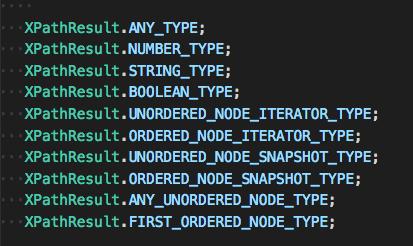
\includegraphics[width=.9\textwidth]{imgs/xpathResult.png}
    \end{center}

\end{frame}

\begin{frame}
    \frametitle{Visualizzare ed Elaborare documenti XML}
    \addtocounter{nframe}{1}
    
    \begin{block}{modello DOM per XML: Xpath Esempio}
        \texttt{result = xmldom.evaluate(}
         \\\texttt{ 'text/back', xmlTEI.documentElement, }
         \\\texttt{ null, XPathResult.BOOLEAN\_TYPE, null);}
    \end{block}

     \begin{block}{modello DOM per XML: Xpath Esempio}
        \texttt{result = xmldom.evaluate(}
        \\\texttt{  'count(text/body/div)', xmldom.documentElement,} 
        \\\texttt{  null, XPathResult.NUMBER\_TYPE, null);}
     \end{block}
     
\end{frame}

\begin{frame}
    \frametitle{Visualizzare ed Elaborare documenti XML}
    \addtocounter{nframe}{1}
    

    \begin{block}{modello DOM per XML: Namespace support}
        \begin{itemize}
            \item Spesso i documenti XML fanno uso di namespace per definire il corretto vocabolario impiegato.
            \item In questa ciscostanza \texttt{XPathEvaluator} deve essere opportunamente impostato.
            \item Nei documenti TEI-XML tutti gli elementi sono parte del namespace \texttt{http://www.tei-c.org/ns/1.0}
        \end{itemize}
        
    \end{block}
     
\end{frame}


\begin{frame}
    \frametitle{Visualizzare ed Elaborare documenti XML}
    \addtocounter{nframe}{1}
    
    %\begin{center}
    %    
\includegraphics[width=.2\textwidth]{../imgs/tei-r.pdf}
    %\end{center}
    %\textit{In parte già disponibili nei moduli TEI di base}

    \begin{block}{modello DOM per XML: Namespace support}
        \begin{itemize}
            \item Un modo per gestire il namespace è attraverso la creazione di un oggetto \texttt{XPathNSResolver}
            \item Invocando il metodo \texttt{createNSResolver()} del documento.
            \item Sfruttando una funzione che, dato un prefisso, restituisce l'URI del namespace. (\texttt{lookupNamespaceURI})
        \end{itemize}
    \end{block}

     
\end{frame}

\begin{frame}
    \frametitle{Visualizzare ed Elaborare documenti XML}
    \addtocounter{nframe}{1}
    
    \begin{block}{modello DOM per XML: Namespace support example}
        \texttt{nsresolver = xmldom.createNSResolver(xmldom.documentElement);} 
        \\\texttt{result = xmldom.evaluate(} \\\texttt{"/tei:TEI/tei:text/tei:front/tei:titlePage",} \\\texttt{xmldom.documentElement, nsresolver, XPathResult.ORDERED\_NODE\_SNAPSHOT\_TYPE, null);}
    \end{block}
     
\end{frame}

\begin{frame}
    \frametitle{Visualizzare ed Elaborare documenti XML}
    \addtocounter{nframe}{1}

    \begin{block}{modello DOM per XML: XSLT support}
        \begin{itemize}
            \item Esiste un oggetto che può essere usato per elaborare fogli di stile XSLT in javascript: \texttt{XSLTProcessor}.
            \item Il promo passo è caricare due documenti DOM: un XML di base, e l'altro XSLT.
        \end{itemize}
    \end{block}

    \begin{block}{modello DOM per XML: XSLT support example}
         \texttt{processor = new XSLTProcessor()} 
         \\\texttt{processor.importStylesheet(xsltdom);}
         \\\text{result = processor.transformToDocument(xmldom);}
    \end{block}
     
\end{frame}

\begin{frame}
    \frametitle{Visualizzare ed Elaborare documenti XML}
    \addtocounter{nframe}{1}
    
    \begin{block}{modello DOM per XML: XSLT support}
        \begin{itemize}
            \item Accanto al metodo \texttt{transformToDocument()} esiste anche il metodo \texttt{transformToFragment()}. 
            \item La ragione per la quale è utile l'utilizzo di tale metodo è per coprire eventuali casi in cui il risultato della trasformazione vuole essere aggiunto ad un ulteriore altro documento DOM.
            \item Tra gli argomenti, infatti, deve essere inserito anche il documento destinatario finale per poter effettuare controlli di consistenza.
        \end{itemize}
    \end{block}     
\end{frame}

\begin{frame}
    \frametitle{Visualizzare ed Elaborare documenti XML}
    \addtocounter{nframe}{1}
    

    \begin{block}{modello DOM per XML: XSLT support example}
        \texttt{fragment = processor.transformToFragment(xmldom, document); }
        \\\texttt{div = document.getElementById('divResult'); }
        \\\texttt{div.appendChild(fragment);}
    \end{block}
     
\end{frame}


\begin{frame}
    \frametitle{Visualizzare ed Elaborare documenti XML}
    \addtocounter{nframe}{1}
    
    %\begin{center}
    %    
\includegraphics[width=.2\textwidth]{../imgs/tei-r.pdf}
    %\end{center}
    %\textit{In parte già disponibili nei moduli TEI di base}

    \begin{block}{modello DOM per XML: XSLT support}
        L'oggetto XSLTProcessor permette di gestire e indicare \textbf{parametri XSLT}.
    \end{block}

    \begin{block}{modello DOM per XML: XSLT support example}
         \texttt{processor = new XSLTProcessor();}
         \\\texttt{processor.importStylesheet(xsltdom);} 
         \\\texttt{processor.setParameter(null, "message", "contenuto del messaggio");} 
         \\\texttt{result = processor.transformToDocument(xmldom);}
    \end{block}
     
\end{frame}

\begin{frame}
    \frametitle{Visualizzare ed Elaborare documenti XML}
    \addtocounter{nframe}{1}
    
    \begin{block}{modello DOM per XML: XSLT support}
        Le istanze dell'oggetto \texttt{XSLTProcessor} possono essere riusate per più trasformazioni e con diversi fogli di stile (efficienza computazionale).
    \end{block}

    \begin{block}{modello DOM per XML: XSLT support example}
        \texttt{processor.importStylesheet(xsltdom); }
        \\\texttt{//do some transformations }
        \\\texttt{processor.reset(); }
        \\\texttt{processor.importStylesheet(xsltdom2); }
    \end{block}
     
\end{frame}

\begin{frame}
    \frametitle{Visualizzare ed Elaborare documenti XML}
    \addtocounter{nframe}{1}

    \begin{block}{modello DOM per XML: concludendo..}
       la tecnologia XML è ad oggi ben supportata dai vari browser, anche se alcune implementazioni differiscono in termini di copertura dello standard e di aderenza ad esso. Esistono comunque tecnologie per avere un supporto cross-browser per le più comuni funzionalità.
    \end{block}
     
\end{frame}



